%%%%%%%%%%%%%%%%%%%%%%%%%%%%%%%%%%%%%%%%%%%%%%%%%%%%%%%%%%%%%%%%%%%%%%%%%%
%%%%%%%%%%%%%%%%%%%%%%%%%%%%%%%%%%%%%%%%%%%%%%%%%%%%%%%%%%%%%%%%%%%%%%%%%%
\clearpage{}
\section{K-factors}
\label{sec:Kfact}

\subsection{\wwa signal K-factor}

Leading-order samples generated by MadGraph5 are used for this analysis. 
Generally, LO calculations can provide a good estimation of cross sections 
and a description of kinematic distributions, but the shortcoming is also 
obvious. Its dependence on the unphysical renormalization and factorization 
scales can result in a large theoretical uncertainty, especially for those 
processes with large logarithms. Therefore, NLO calculations are important 
for precise analysis. In an experimental analysis, generally one can use a 
K-factor, which is defined as the ratio of the NLO to LO cross section for 
a given process, to estimate the NLO effect. However, its dependence on the 
renormalization and factorization scales, as well as the parton distribution
functions (PDFs), should result in large uncertainties. Moreover, the NLO 
corrections can also lead to shape changes in kinematic distributions, 
especially when tight cuts are applied. Thus, one needs to make a careful 
examination to get a reasonable K-factor.

The emerging package aMC@NLO ~\cite{Frederix:2011zi,Frederix:2011qg} 
implements automatic event generation with NLO accuracy, which is a great 
improvement of MC hard events generation. However, we do not use the NLO 
samples for our analysis. Instead, we investigated the K-factor distribution
as a function of the photon $p_{T}$, which gives us reasonable K-factors for
our \wwa samples. 

For our analysis, 200k \wwa signal events, without W decays, are first 
generated using aMC@NLO. Then the samples are passed to 
HERWIG~\cite{Corcella:2000bw} to do parton shower. In the framework of 
aMC@NLO, theoretical uncertainties can also be obtained through a 
process-independent technique introduced in Ref.~\cite{Frederix:2011ss}, 
which allows aMC@NLO to compute scale and PDF uncertainties in a fully 
automated way and at no extra CPU-time cost. The default renormalization and
factorization scales are set equal to the sum of transverse masses of all 
final state particles and partons. To get scale dependence, we vary the 
$\mu_R$ and $\mu_F$ independently, considering the set of 
$(\mu_R,\mu_F) = (\kappa_R \mu_R,\kappa_F \mu_F)$, with \\ 
%%
$(\kappa_R,\kappa_F) = (1, 1), (1/2, 1/2), (2, 2)$\\
%%
and the overall scale uncertainty is the maximum deviation of all the sets.
The PDF uncertainty is estimated following the method (asymmetric Hessian) 
illustrated in Ref.~\cite{Martin:2009iq}. The 
$MSTW2008nlo68cl$~\cite{Martin:2009iq} PDF sets are used for this analysis 
which contains 20 pairs to compute PDF uncertainties.

To make the result close to the experimental analysis, some basic cuts
have been applied for the samples. $p_{T_{\gamma}} > 10 \text{GeV}$
and $|\eta_{\gamma}| < 2.5$ have been used for both LO and NLO
calculation.  As for photon isolation cut, the cone approach is not
infrared safe for NLO calculation. Therefore, we adopted the isolation
cut introduced in Ref.~\cite{Frixione:1998jh, Bozzi:2009ig}instead: if
$i$ is a parton with transverse energy $E_{T_{i}}$ and a separation
$R_{i_{\gamma}}$ with a photon of transverse momentum $p_{T_{\gamma}}$,
then the event is accepted only if:

\begin{equation}
\sum_i E_{T_i} \theta ( \delta - R_{i{\gamma}} ) \leq p_{T_{\gamma}} \frac{ 1 - cos \delta }{ 1 - cos \delta_0 } \text{    } ( \text{  for all } \delta \leq \delta_0 )
\label{nloacut}
\end{equation} 

where $\delta_0$ is fixed to be 0.7. 

\begin{figure}[]{
\centering
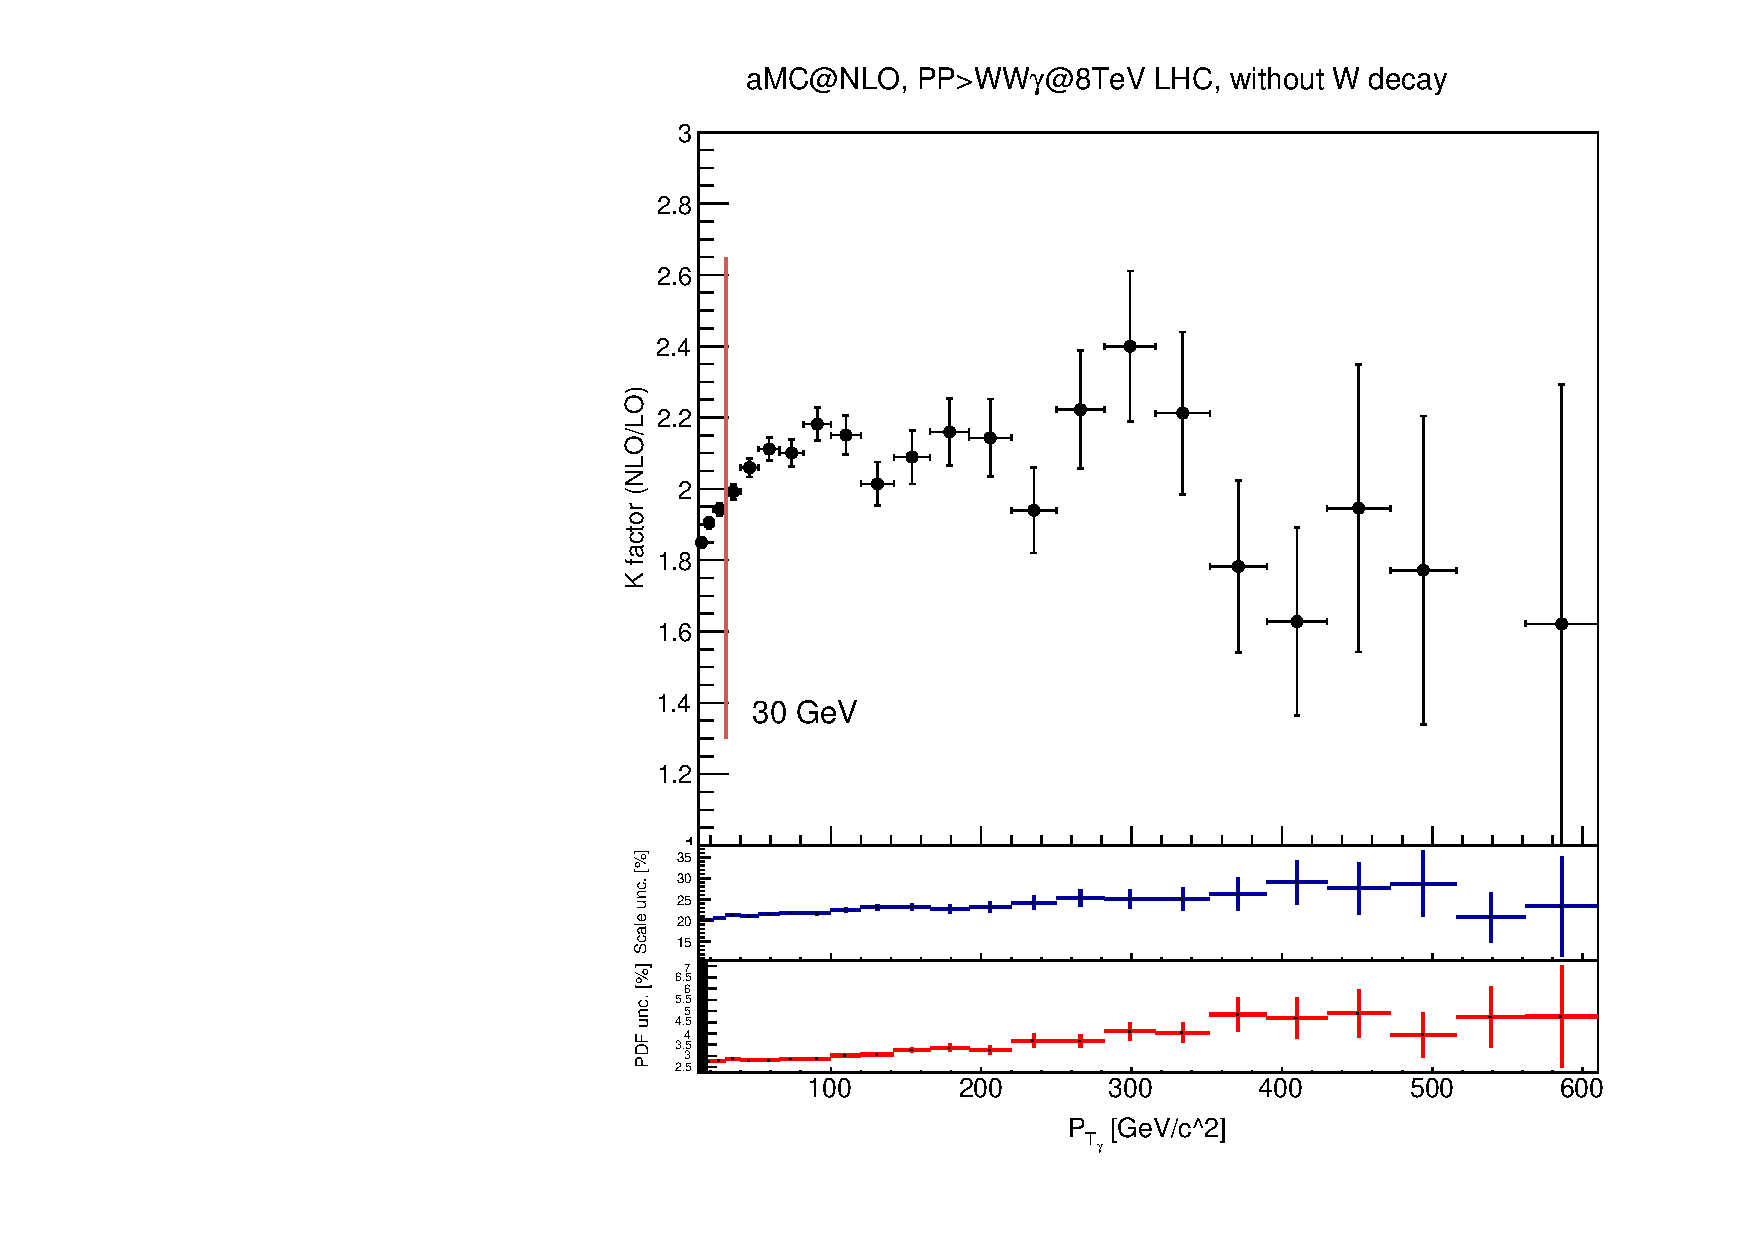
\includegraphics[width=0.4\textwidth]{figs/kwwa_pt.pdf}
\caption{\label{k-wwa} \wwa signal sample K-factor distribution as a function of $p_{T_{\gamma}}$.}}
\end{figure}

In Figure~\ref{k-wwa}, the K-factor distribution is quite flat; we use a Binned Likelihood method fit to a constant to get the value of the K-factor. 
Therefore, the K-factor value, with scale and PDF uncertainties, we use for 
the SM signal sample is 2.09812 $\pm$ 0.302029\% (stat.) $\pm$ 23.4256\% 
(scale) $\pm$ 3.55719\% (PDF).

\newpage
\subsection{aQGC K-factor}
\label{sec:aQGC_Kfac}

The MC samples for aQGC study are generated as SM WV$\gamma$ with added aQGC.
K-factor for two values of $a_{0}^{W}/\Lambda^{2}$ and $a_{C}^{W}/\Lambda^{2}$ are computed 
as function of the photon $p_{T}$ and show on Figure~\ref{k-Awwa}. At low photon $p_{T}$ the 
K-factor resembles the SM WW$\gamma$ K-factor, while with the increase of the photon $p_{T}$, most of 
the contributions are from the quardrilinear diagrams, and one can expect that the value will be similar to the Drell Yan processes.
The K-factor $p p \rightarrow W^{+}$ and $ p p \rightarrow Z$ processes have been also calculated , and the results turned out to be 
1.185 and 1.184. As can be seen in Figure~\ref{k-Awwa}, the aQGC K-factor levels at approximately 1.185 when the
photon $p_{T}$ is greater than 300 GeV/c. The exact behavior of the K-factor at low photon $p_{T}$ for the SM WW$\gamma$ with added aQGC 
depends on type of the aQGC parameter and its value. On Figure~\ref{k-Awwa} is shown the K-factor for two different aQGC parameters, 
while on Figure~\ref{k-diffvalue} is shown the K-factor for two different values of the same aQGC parameters, namely 
$a_{0}^{W}/\Lambda^{2}$.

In this study we define as visible aQGC signal only the contribution, which is originated from the anomalous quardrilinear diagrams.
The limit-setting machinery, discussed
in Section~\ref{sec:aQGClim}, uses a signal input distribution which is the
difference between the SM WV$\gamma$ with added aQGC and SM WV$\gamma$ only photon $p_{T}$ distributions (refer to as "aQGC-SM").
Since virtually all events with a photon $p_{T}$ above 300 GeV/c are predicted to
be from aQGC in our analysis, then the input distribution should reflect the
K-factor of 1.185 only. To accomplish this, when preparing the input file 
for the limit setter, we do not use a K-factor for either the SM or aQGC 
samples in the aQGC-SM subtraction. With the resulting aQGC-SM distribution
being primarily high photon $p_{T}$ events, and aQGC in nature, then we
apply the K-factor of 1.185. Since there are some remaining low photon 
$p_{T}$ aQGC events in the aQGC-SM distribution, we are applying a constant
K-factor across the board. An illustration of the resulting K-factor from such procedure is shown on Figure~\ref{k-pureaqgc}.
Photon $p_{T}$ distributions for aQGC-SM LO and NLO samples are shown on \ref{k-pureaqgc}a, while the resulting K-factor is 
shown on \ref{k-pureaqgc}b. 

\begin{figure}[]{
\centering
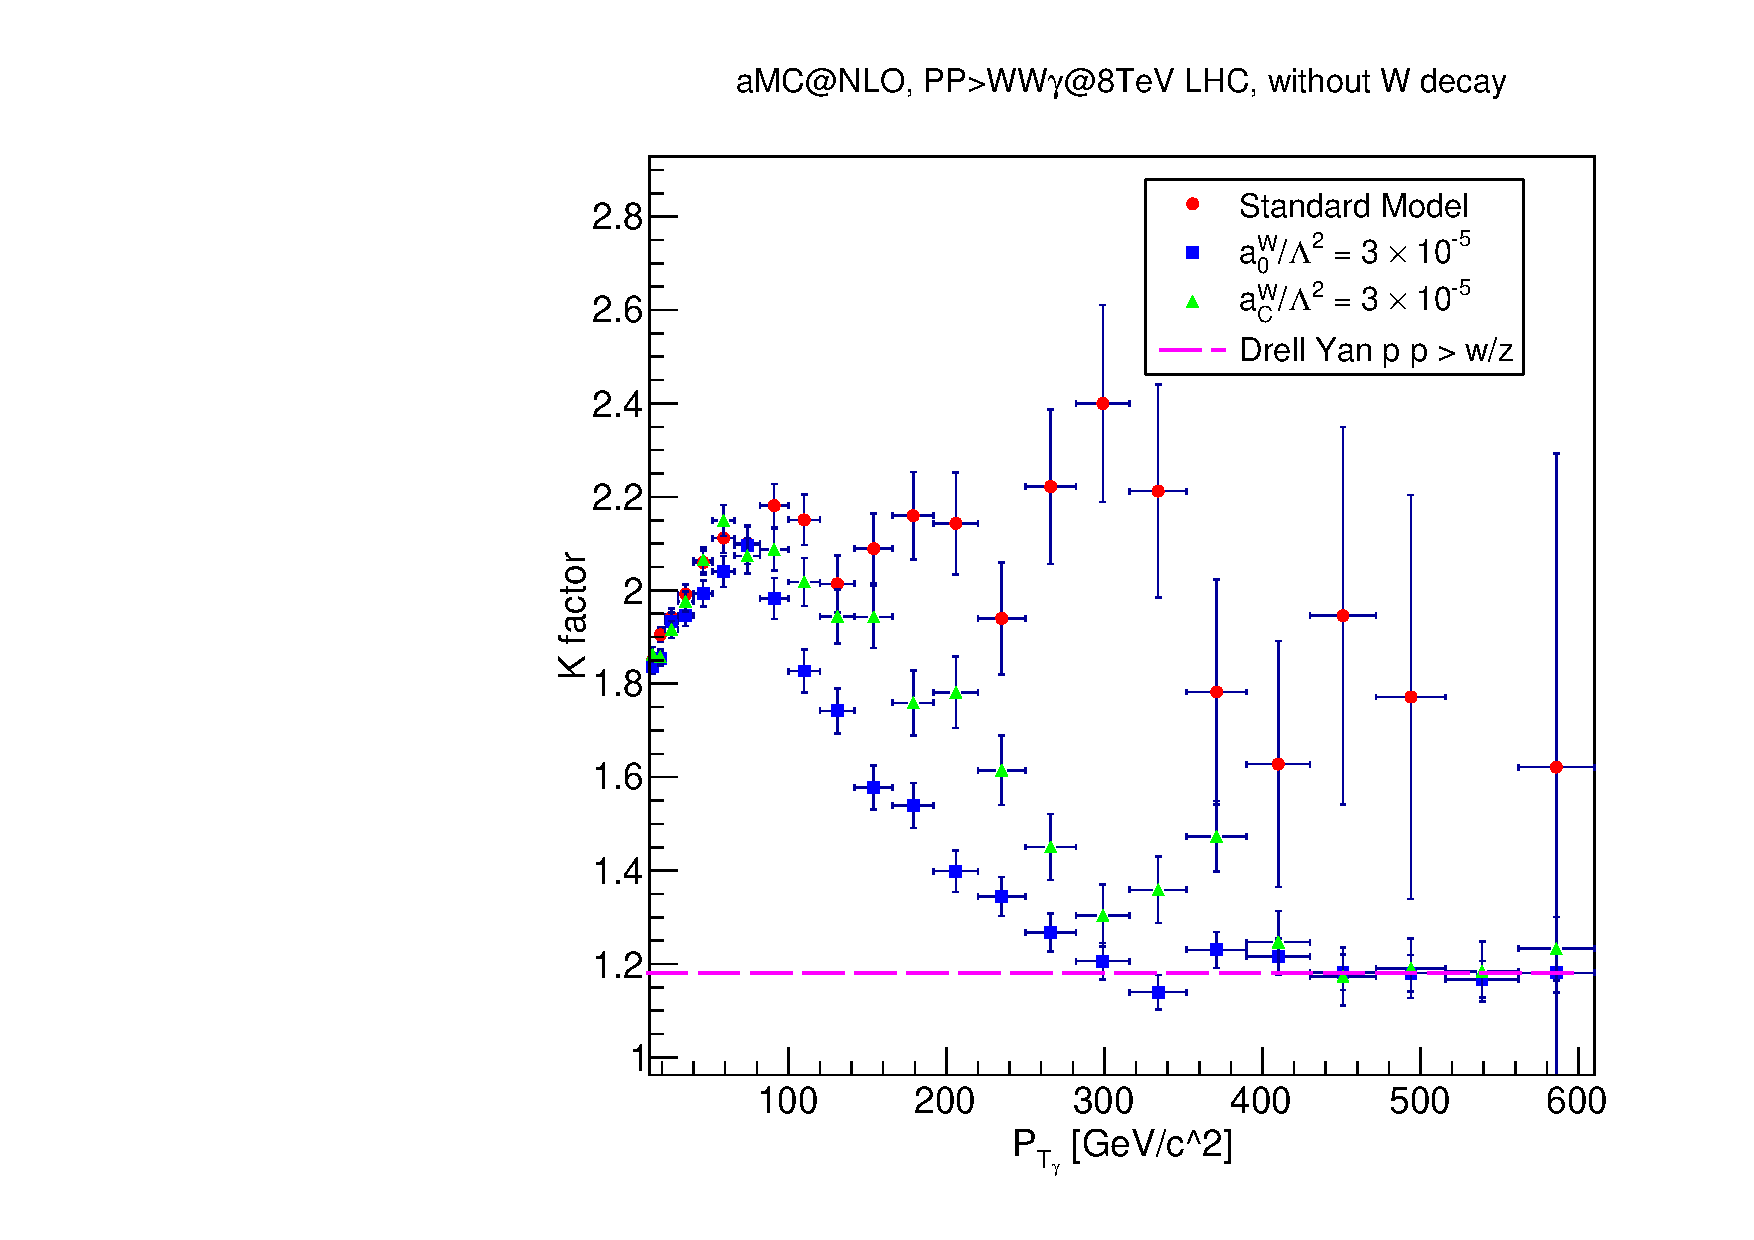
\includegraphics[width=0.4\textwidth]{figs/kAwwa_pt.pdf}
\caption{\label{k-Awwa} \wwa signal aQGC sample K-factor distribution as a function of $p_{T_{\gamma}}$}}
\end{figure}

\begin{figure}[]{
\centering
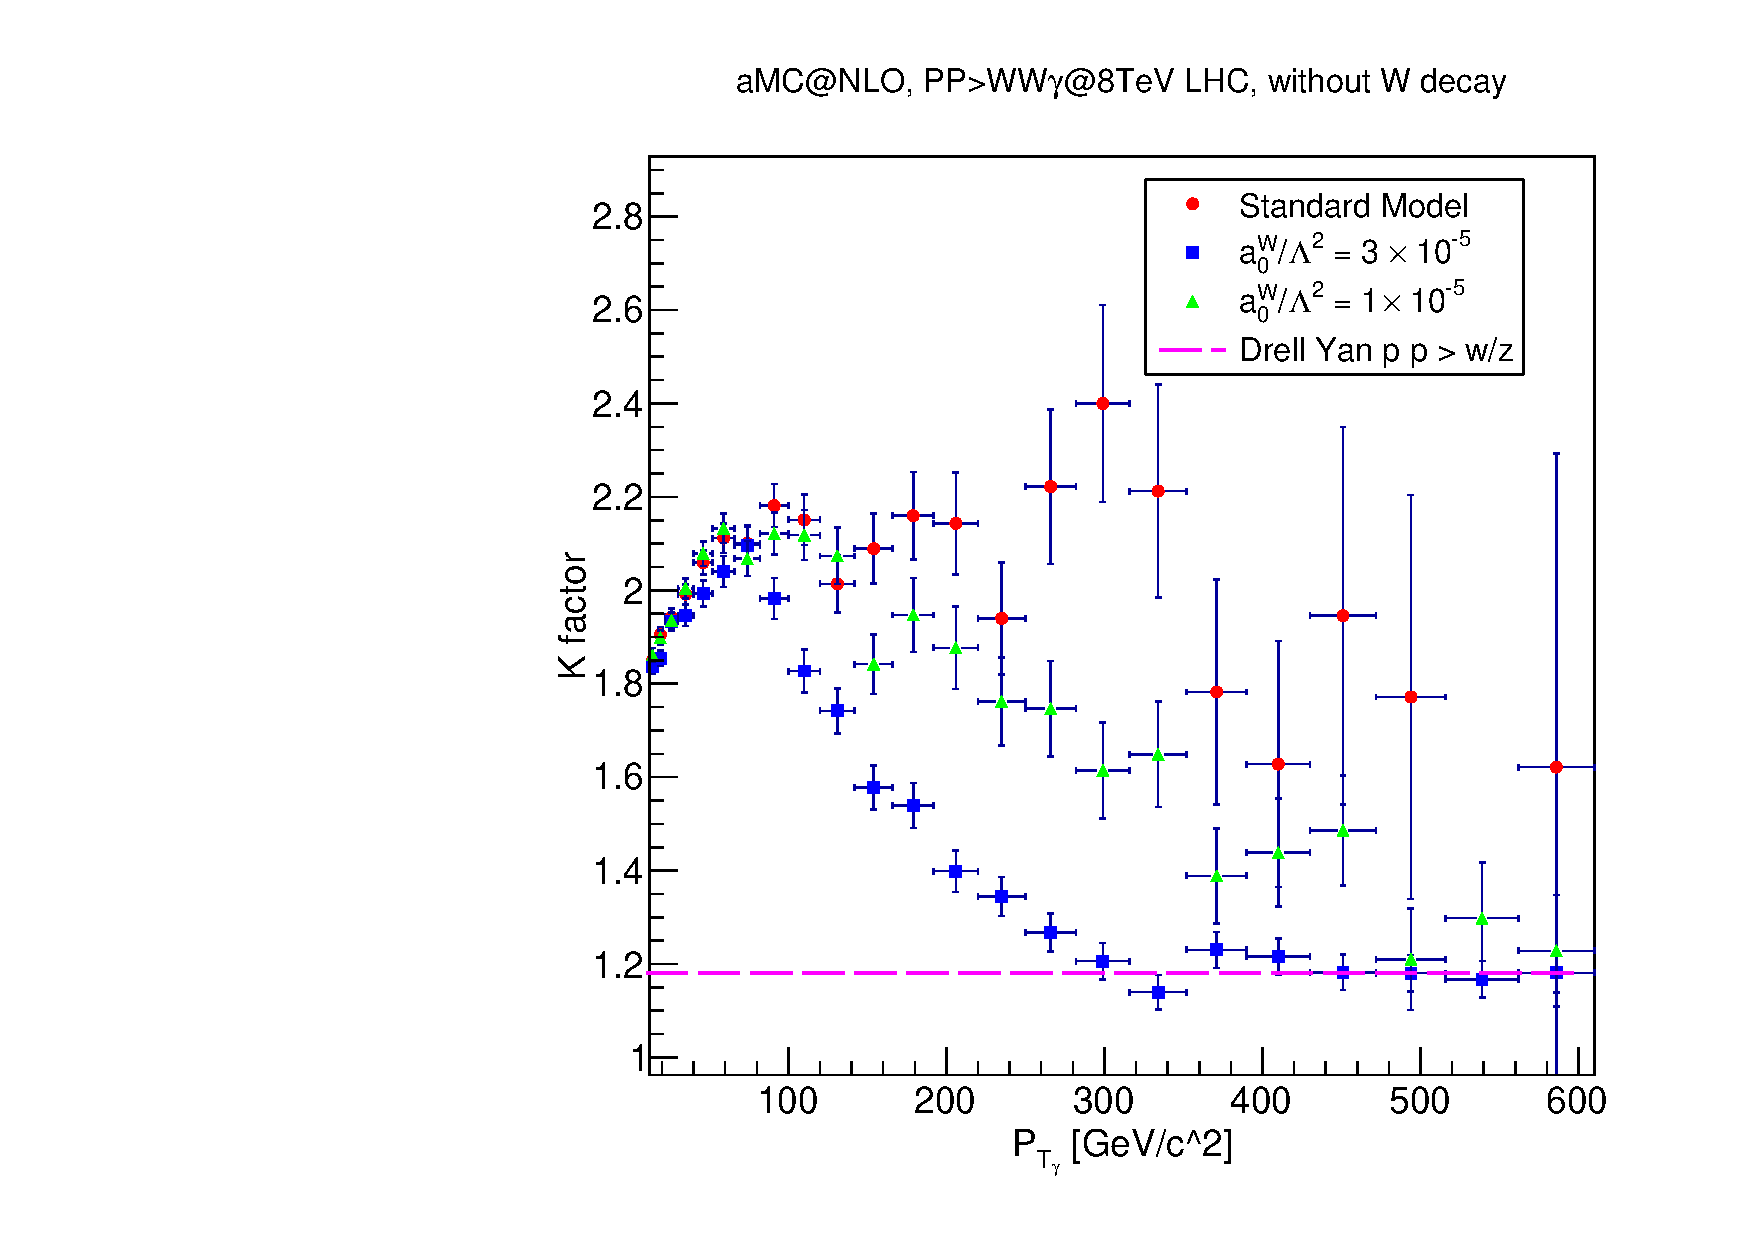
\includegraphics[width=0.4\textwidth]{figs/diffvalue_Kfactor.pdf}
\caption{\label{k-diffvalue} \wwa signal aQGC sample K-factor distribution with different $a_0^W/\Lambda^2$ values }}
\end{figure}

\begin{figure}[]{
\centering
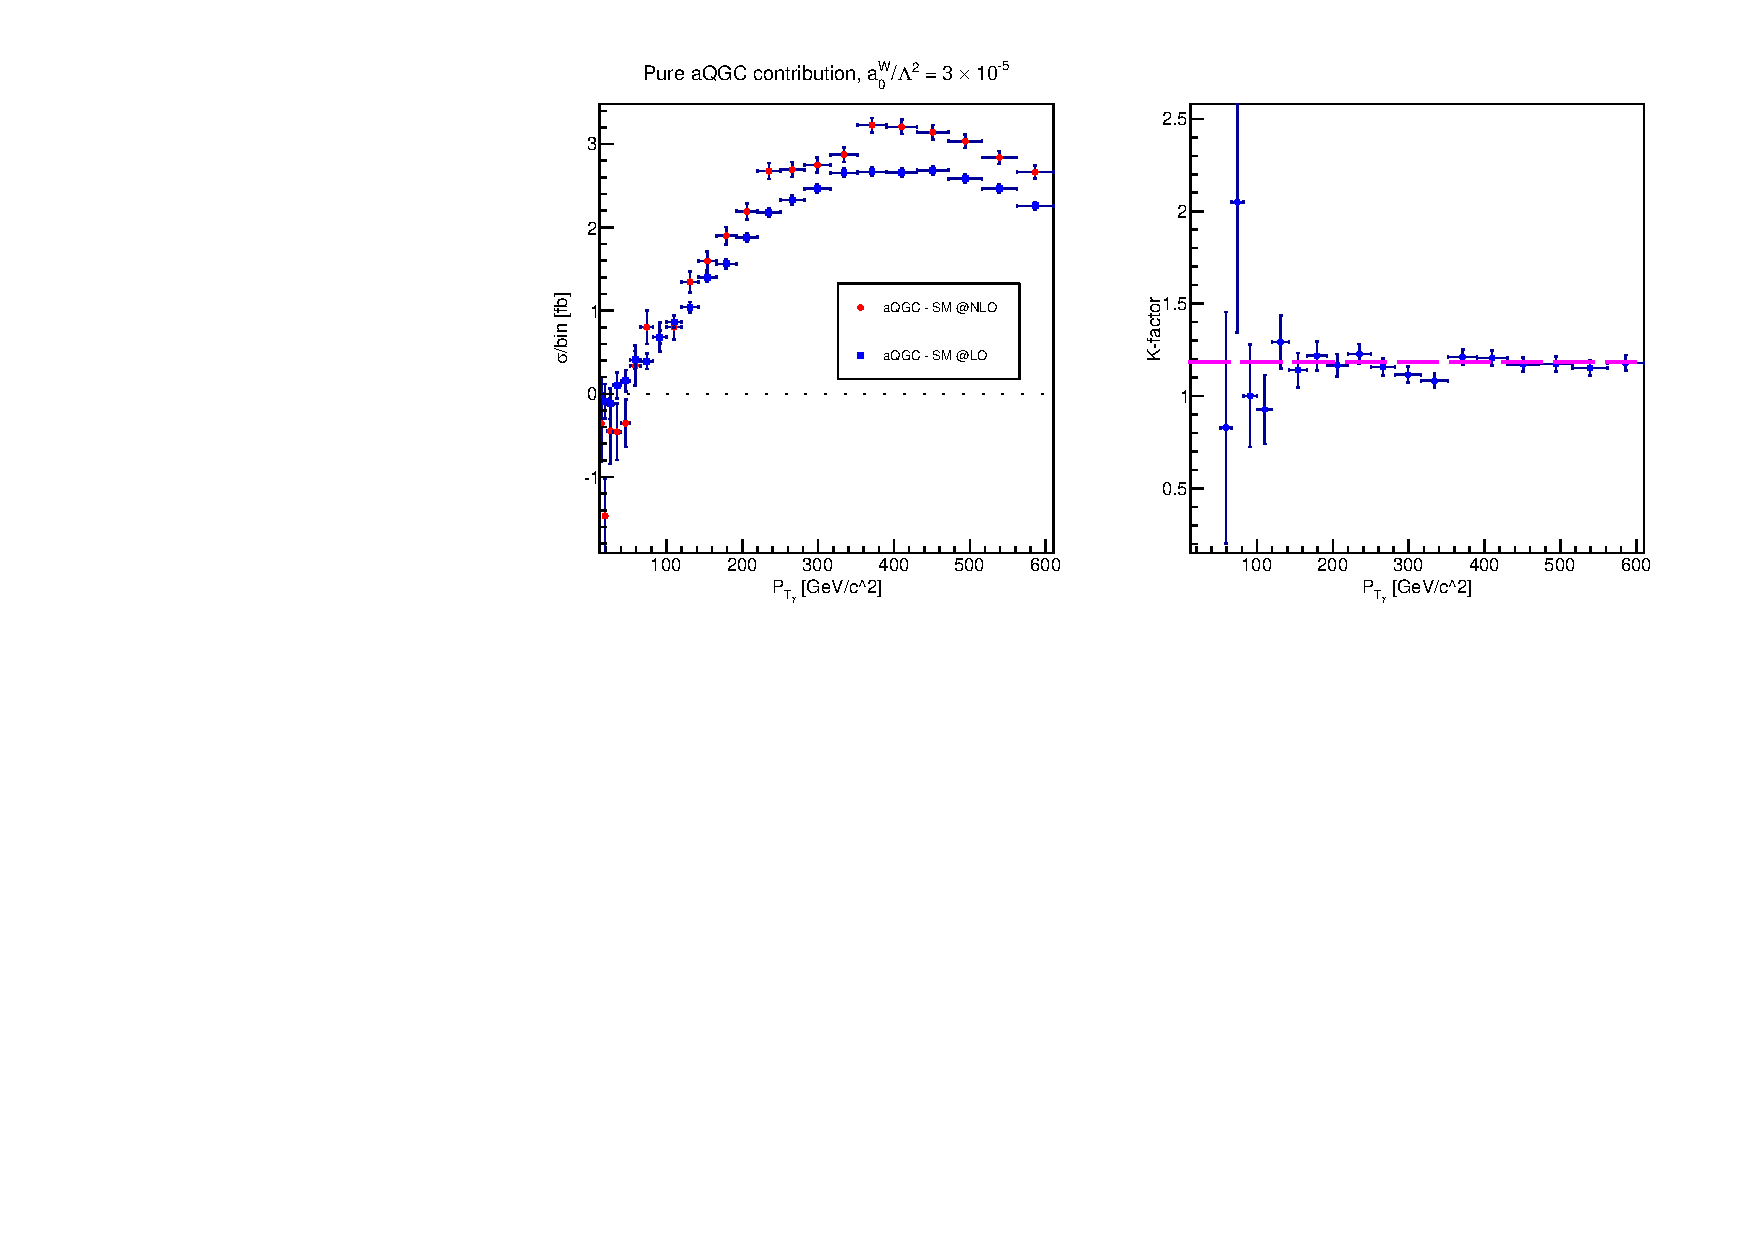
\includegraphics[width=0.8\textwidth]{figs/pureaqgc_Kfactor.pdf}
\caption{\label{k-pureaqgc} \wwa signal aQGC-SM $p_{T_{\gamma}}$ distribution (left) and K factor distribution (right), with $a_0^W/\Lambda^2 = 3 \times 10^{-5} GeV^{-2}$}}
\end{figure}

As additional cross check we have calculated the K-factors for SM WV$\gamma$ with added aQGC for all values of the $a_0^W/\Lambda^2$ parameter and 
re-calculated the limits on this parameter. The limits are shown in Section~\ref{sec:aQGClim}, while the conclusion is that with either of the 
described two procedure we arrive to the same constrains on the aQGC values. Thus we have chosen to used the methods with constant Drell Yan like K-factor for 
aQGC-SM, as the precise calculation of the K-factors for all values of all studied aQGC parameter will take vary long time.
In this last cross check we have used the following function to fit the K-factor shape for SM WV$\gamma$ with added aQGC:
\begin{equation}
\begin{cases}
slp \cdot x + ( top - slp \cdot cuta), \text{     } x \leq cuta  \\
(top-1.185) \cdot exp(-tau \cdot (x-cuta)) + 1.185, \text{     } x > cuta 
\end{cases}
\label{k-fitfunc}
\end{equation}
where the slp, top, cuta, tau are fit parameters and x represent the $p_{T_{\gamma}}$. K-factors and the fit are shown on  
Figure~\ref{k-fitshape} for $a_0^W/\Lambda^2 = p \times 10^{-5} GeV^{-2}$, where $p= 2,3,5.


\begin{figure}[]{
\centering
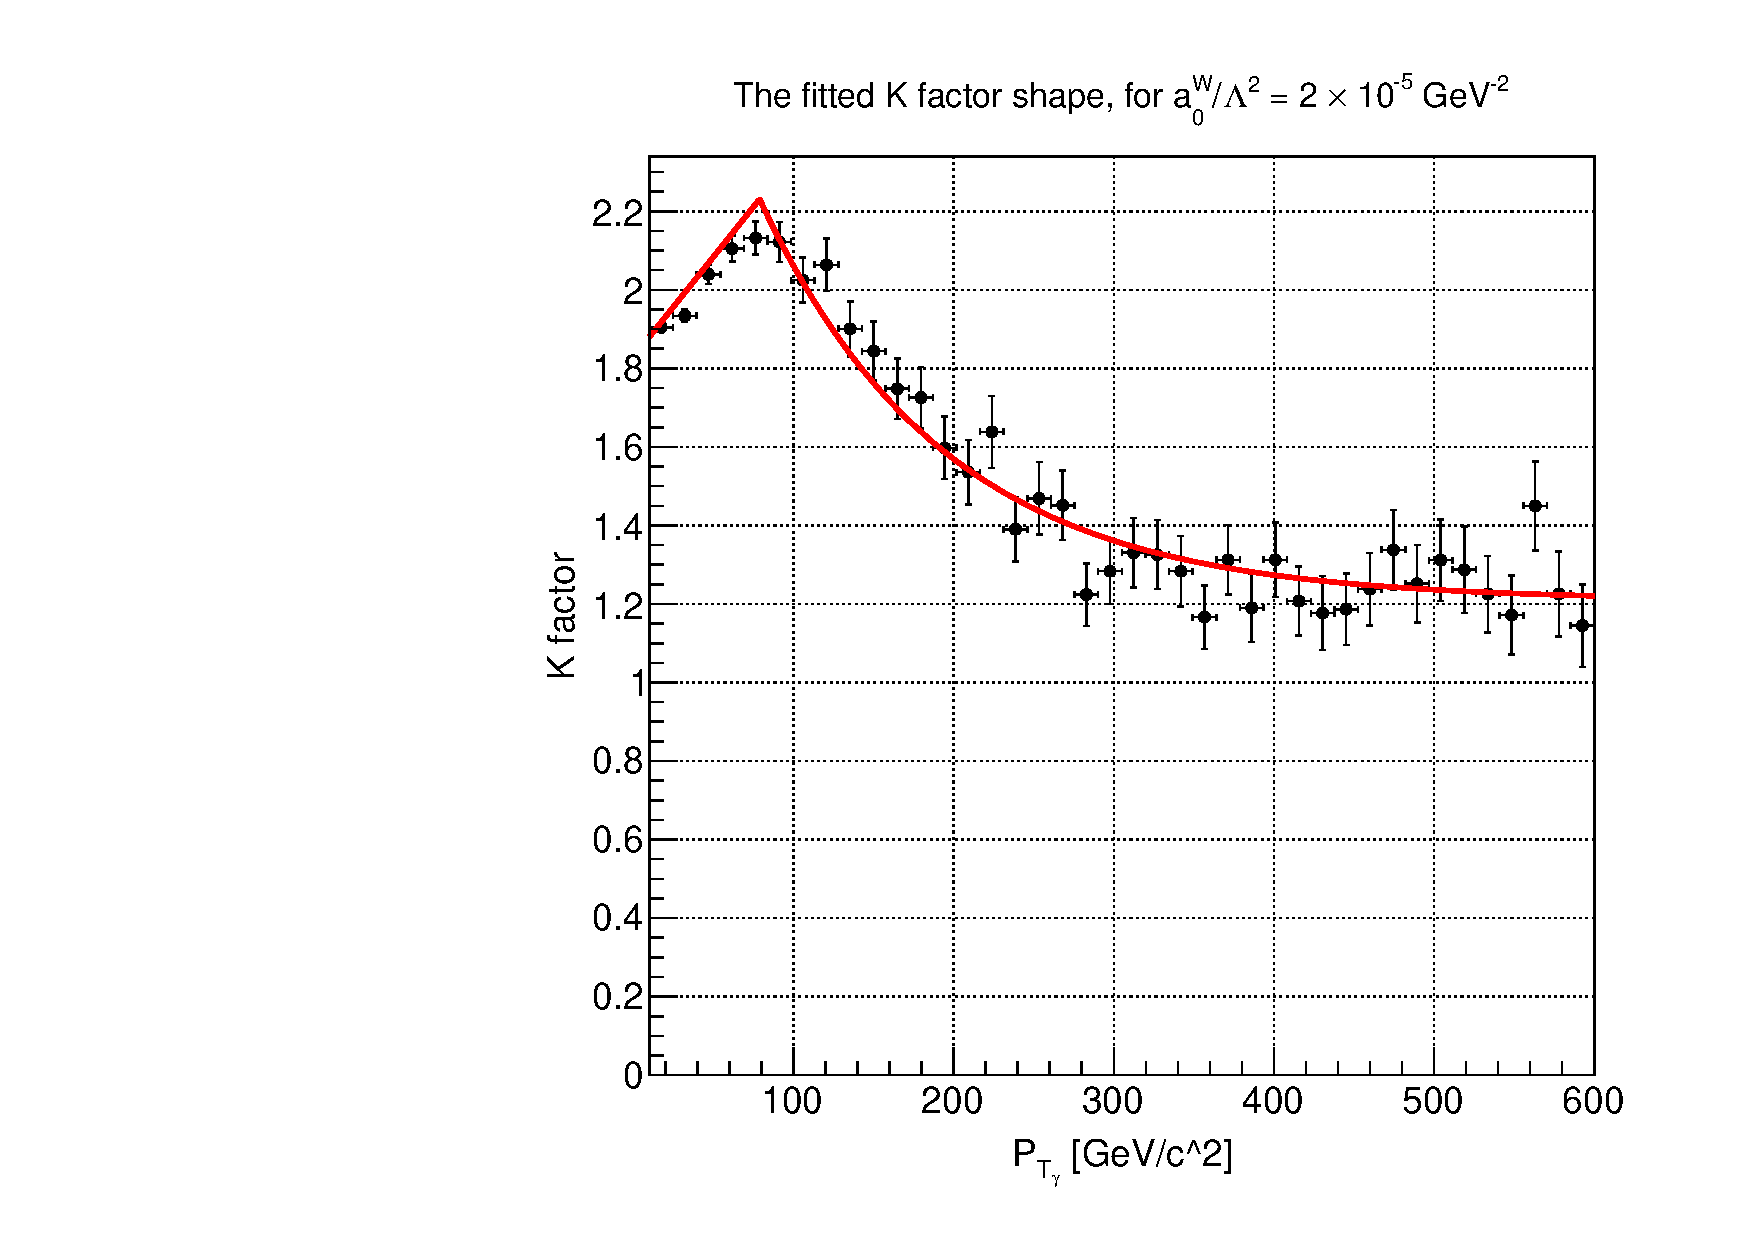
\includegraphics[width=0.4\textwidth]{figs/a0w_kshape_p2.pdf}
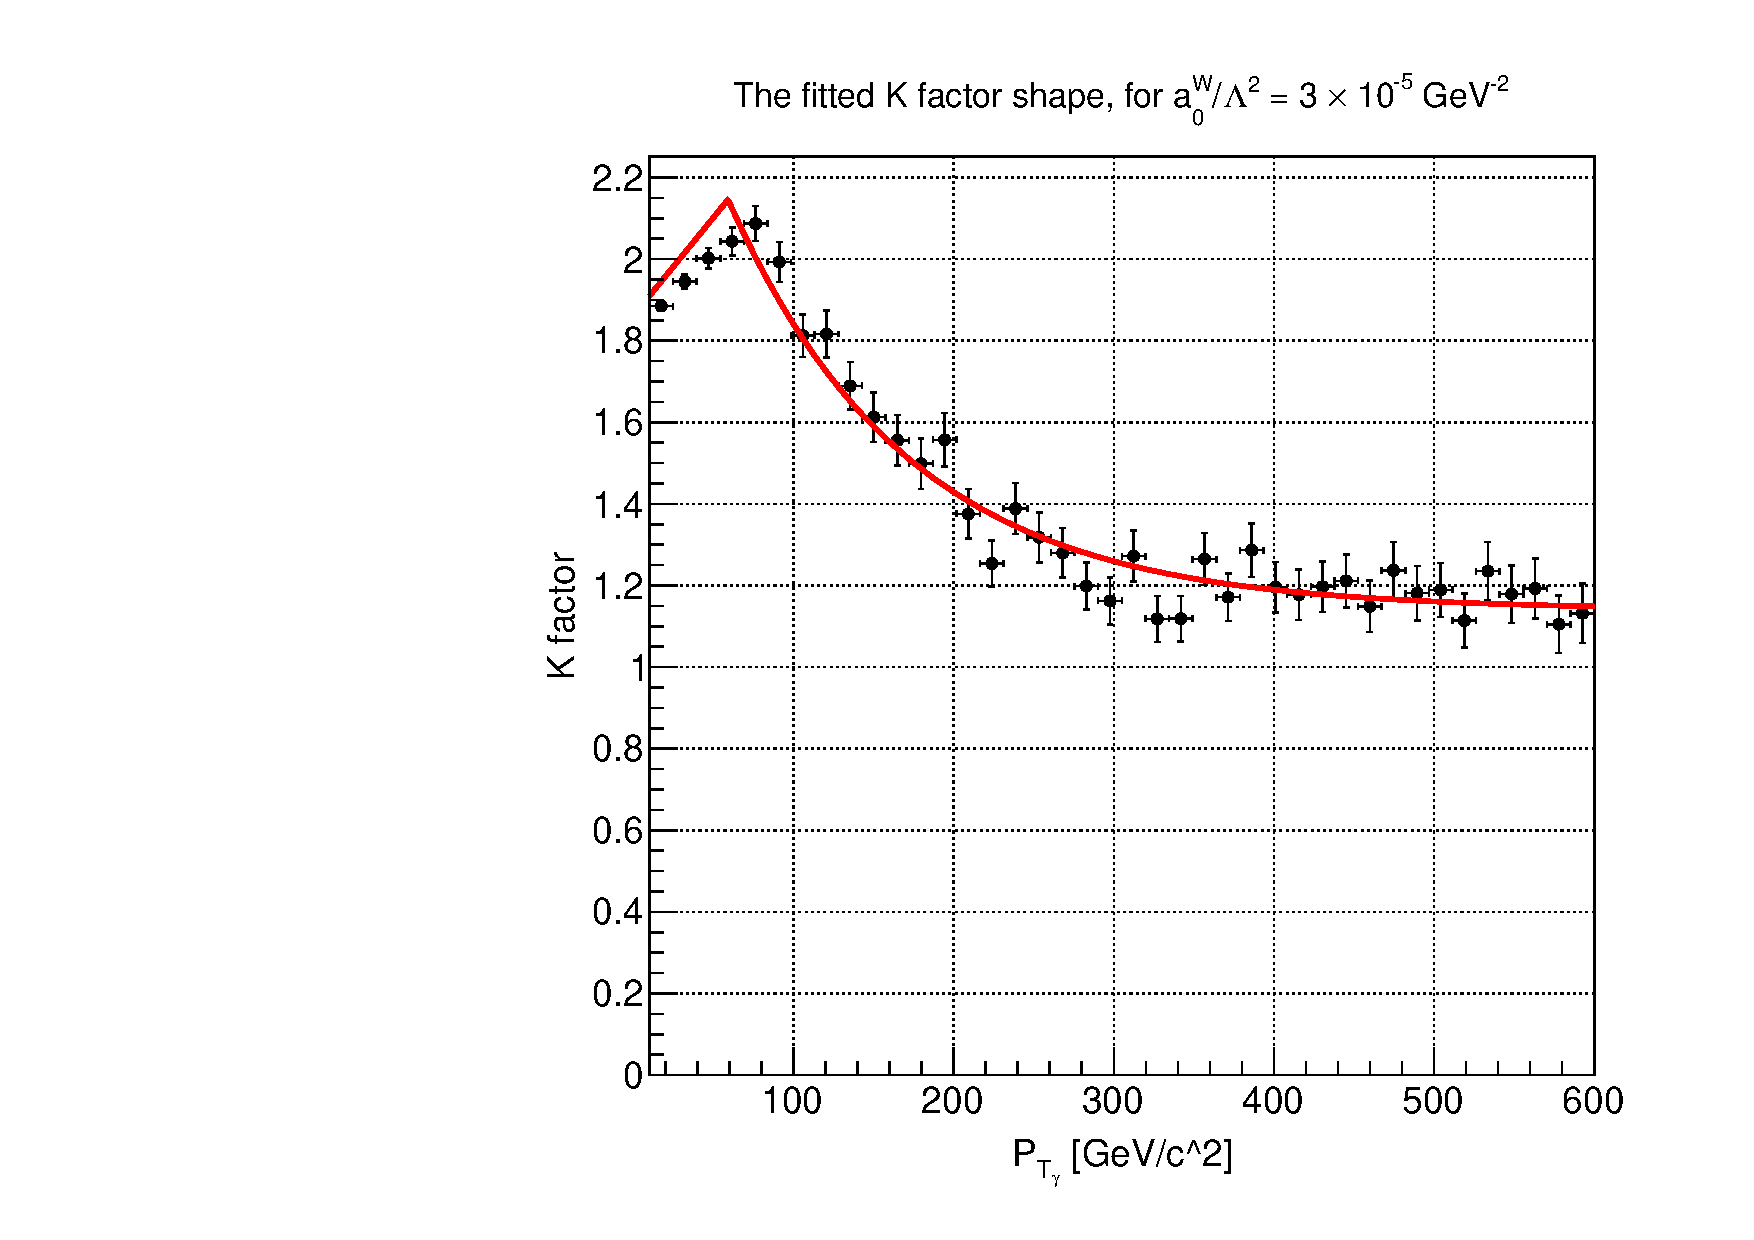
\includegraphics[width=0.4\textwidth]{figs/a0w_kshape_p3.pdf}
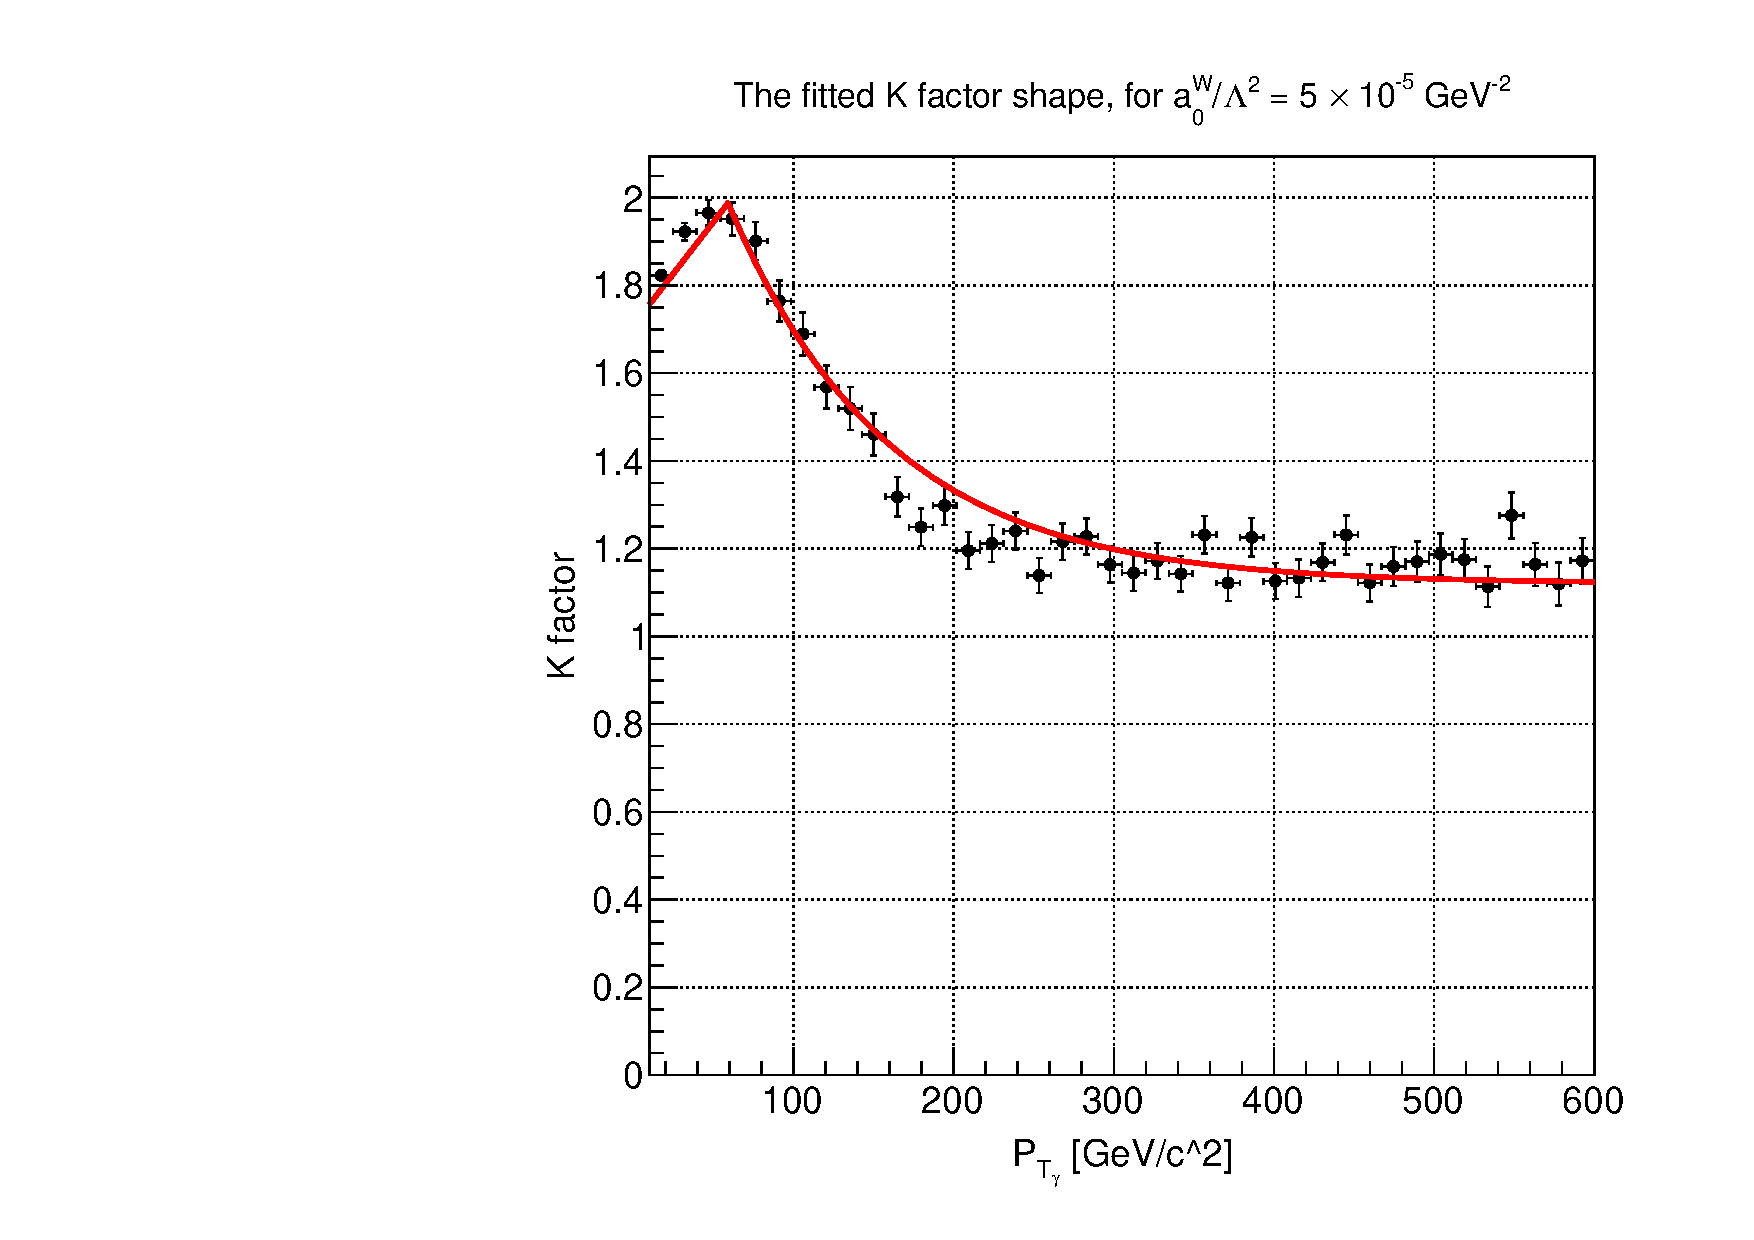
\includegraphics[width=0.4\textwidth]{figs/a0w_kshape_p5.pdf}
%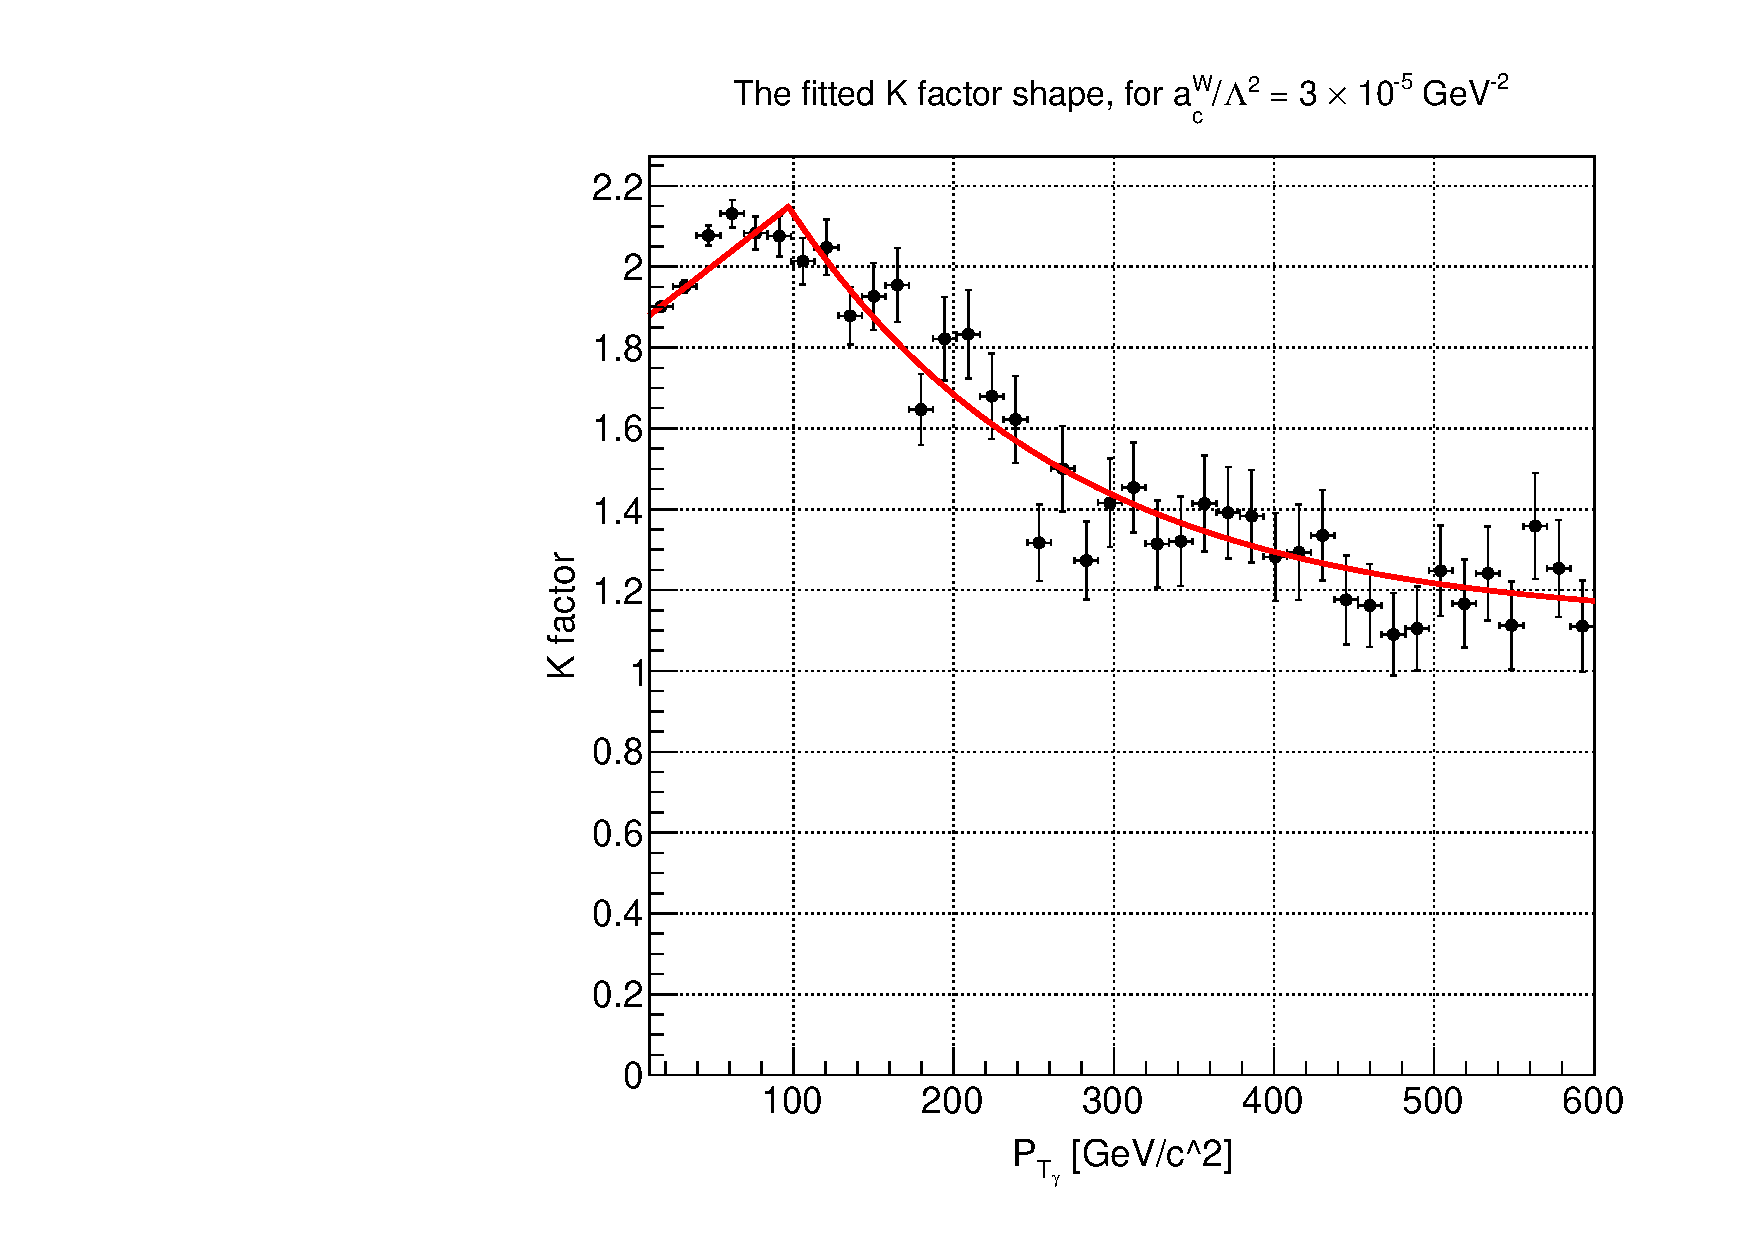
\includegraphics[width=0.4\textwidth]{figs/acw_kshape.pdf}
\caption{\label{k-fitshape} K factor shape fitted with function ~\ref{k-fitfunc}, for $a_0^W/\Lambda^2 = 2,3,5 \times 10^{-5} GeV^{-2}$  }}
\end{figure}


\subsection{W$\gamma$ + jets background estimation}

In order to estimate the normalization of the major background
W$\gamma$+jets, we used a data-driven technique.
%% The method involved analyzing sideband distributions in the W$\to$jj
%% mass spectrum in data.
%% These sidebands lie outside of a 70-100 GeV $M_{W,Z}$ window,
%% and in addition include all other normalized Monte Carlo background
%% and signal contributions, of which there was less than 0.6\% signal
%% contamination.
The background normalization in the signal region is extracted with a
binned maximum likelihood fit to the dijet invariant mass
distribution $m_{jj}$ of the two leading jets. The signal region
corresponding to the W and Z mass windows, $70 GeV < m_{jj} <
100 GeV$, is excluded from the fit.  The W$\gamma$+jets shape is
taken from simulation.  The overall normalizations of the
W$\gamma$+jets and fake photon components are allowed to vary in the
fit.  All other backgrounds, which contribute less than 10\% to the
total, are based on simulation and are fixed to their SM expectations
with uncertainties.  The multi-jet background shape is derived from
data by relaxing lepton isolation and identification requirements. Its
contribution to the total number of events is evaluated from a
separate two-component likelihood fit to the \MET
distribution, and fixed in the $m_{jj}$ fit according to this
fraction within uncertainties~(\cite{CMS-AN-12-224}, Section 11).
Normalization for the W$\gamma$+jets is measured to be $1.099 \pm
0.073$ for muons and $1.074 \pm 0.085$ for electrons. The quality of
the fit is illustrated on Figure ~\ref{fig:wapjets_kfct}

Table~\ref{tab:MCxsec} summarizes
the K-factors and cross sections used for each Monte Carlo sample,
as well as the treatment of all backgrounds in the fit.

\begin{table}[htb]
\centering
\scalebox{0.8}{
  \begin{tabular}{|l|c|c|l|}
  \hline
  MC Sample & K & $\sigma$ [pb] & External constraint on normalization \\
   &  &  & used in W$\gamma$+jets fit \\
  \hline
  \hline
  SM WW$\gamma$            & 2.1        & 0.02771    & Fixed \\
  SM WZ$\gamma$            & 2.1        & 0.00578008 & Fixed \\
  anomalous WWV$\gamma$    & 1.185      & -          & NA    \\
  W$\gamma$+jets           & 1.10(mu),1.07(el)  & 9.37246    & Unconstrained \\
  Fake photon              & from data  & -          & Constrained \\
  Multi-jet                & from data  & -          & Fixed: \MET fit in data $\pm$ 50\% (100\%) for electrons (muons) \\
  Z$\gamma$+jets           & 1          & 0.63196    & Fixed \\
  t$\overline{t}\gamma$    & 1          & 1.44       & Fixed \\
  Single Top (s-channel)   & NLO        & 3.89394    & Fixed \\
  Single Top (t-channel)   & NLO        & 55.531     & Fixed \\
  Single Top (tw-channel)  & NLO        & 11.1773    & Fixed \\
  Single Top (ps-channel)  & NLO        & 1.75776    & Fixed \\
  Single Top (pt-channel)  & NLO        & 30.0042    & Fixed \\
  Single Top (ptw-channel) & NLO        & 11.1773    & Fixed \\
  \hline
  \end{tabular}}
  \caption{List of backgrounds, the theoretical K-factors and cross
  sections used for MC-based backgrounds, and how they are treated in
  the background normalization template fit. The data-driven K-factor
  for W$\gamma$+jets sample is listed for both the muon and electron
  channels.}  \label{tab:MCxsec}
\end{table}

%% Examples of the $m_{jj}$ fit are shown in
%% Figure~\ref{fig:mjj_mH350} for the muon channel, with selections
%% optimized for Higgs mass hypotheses 190\GeVnn, 300\GeVnn, and
%% 500\GeVnn. The uncertainties in the normalization obtained from the
%% fit are propagated to the limit calculation as a systematic
%% uncertainty.  The signal $m_{jj}$ distributions are shown in
%% figure~\ref{fig:mjj_signals}.

\begin{figure}[b]
   \begin{center}
      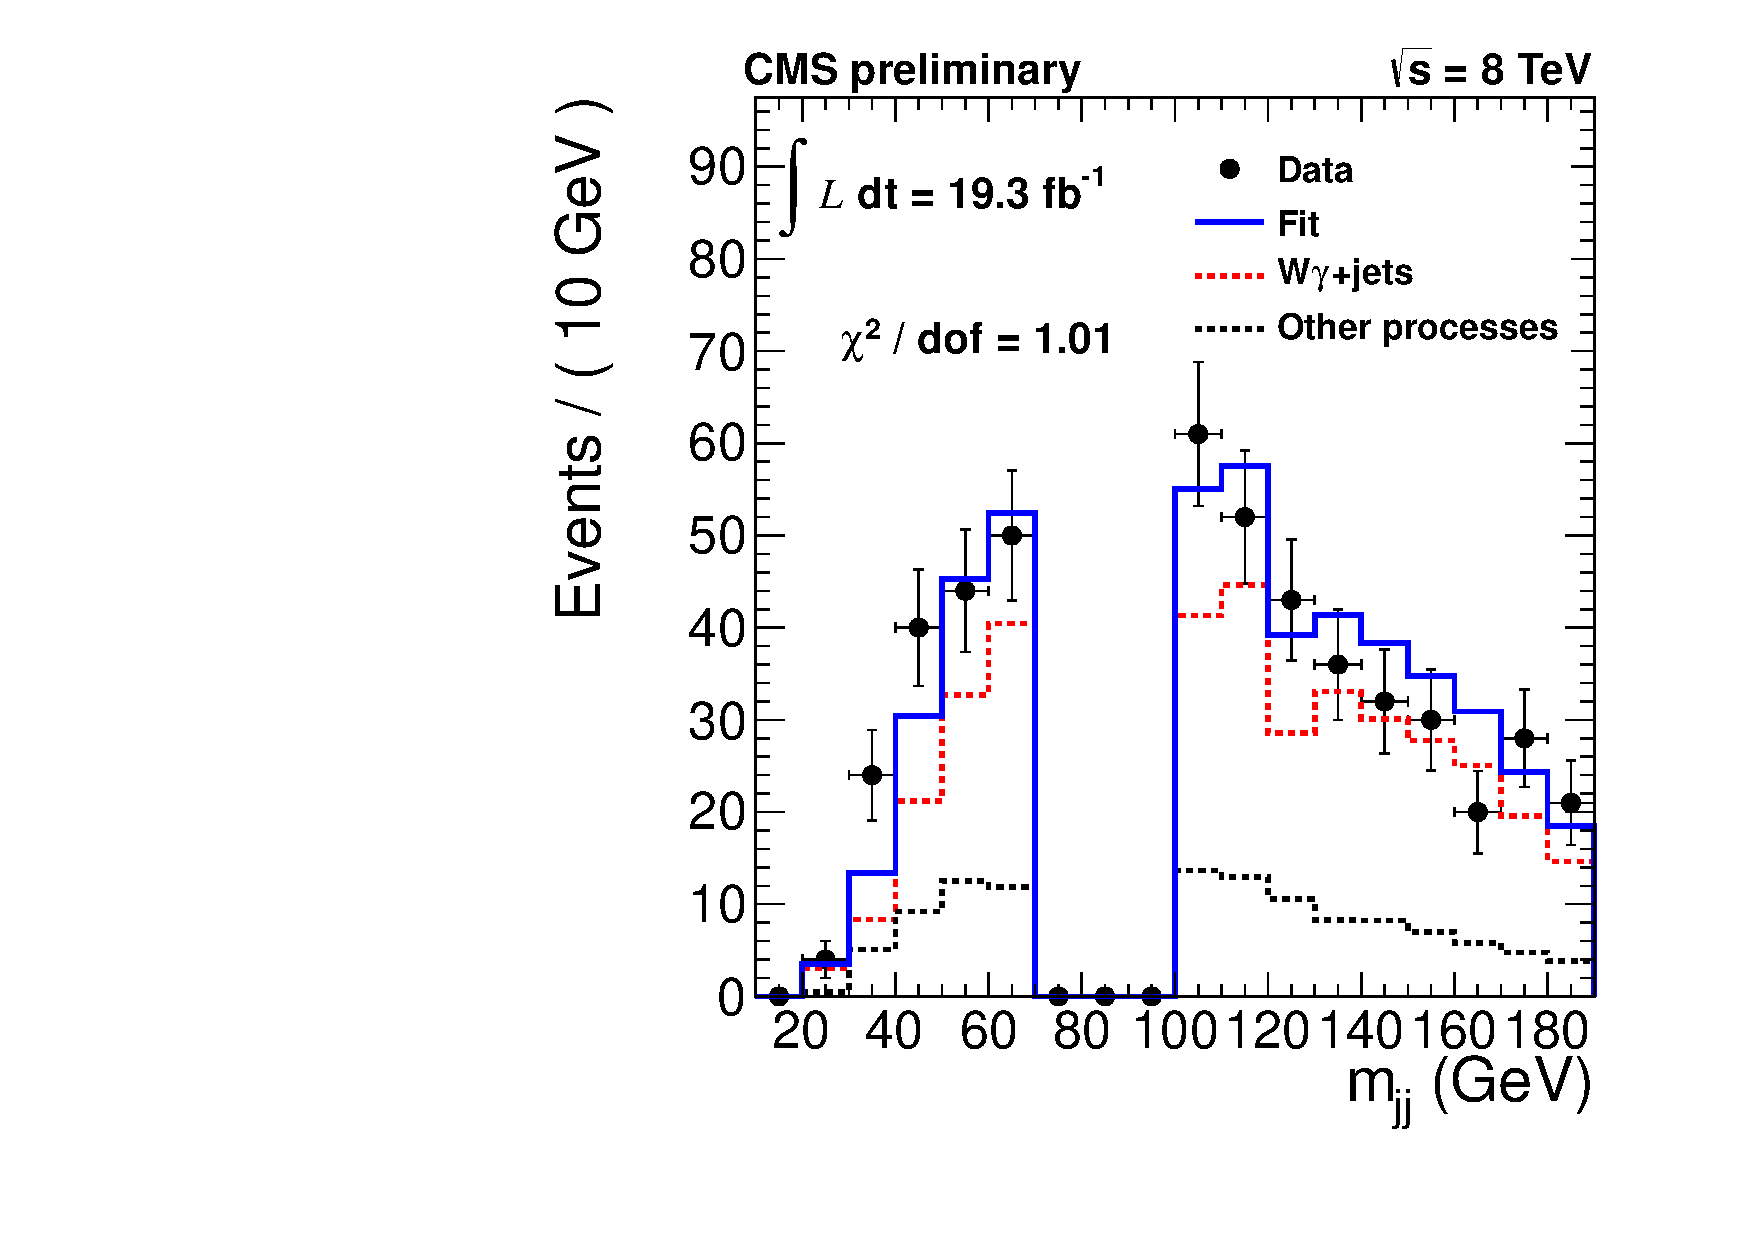
\includegraphics[width=0.4\textwidth]{figs/mu_mjj1.pdf}
      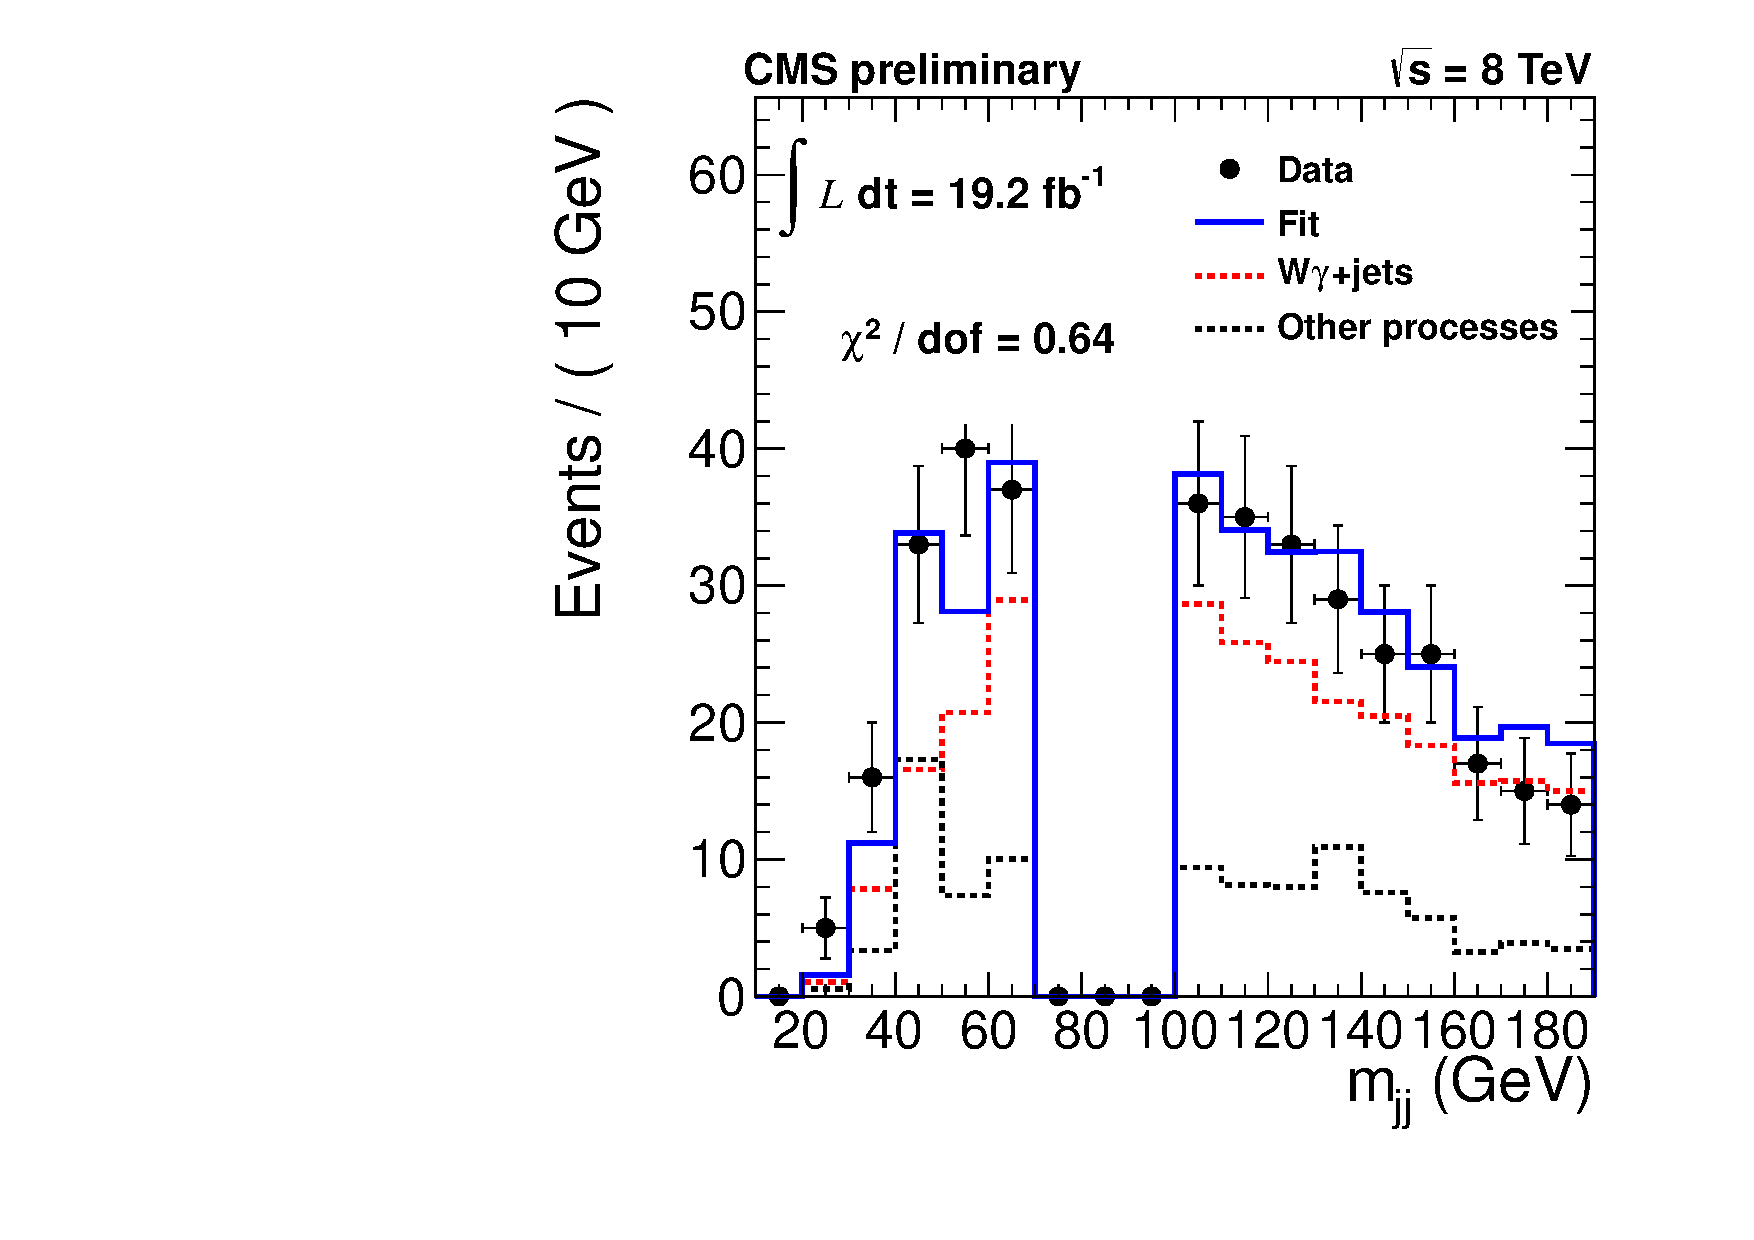
\includegraphics[width=0.4\textwidth]{figs/el_mjj1.pdf}
      \caption{Data and MC dijet mass sidebands used to estimate the data-driven W$\gamma$+jets K-factor.}
      \label{fig:wapjets_kfct}
   \end{center}
\end{figure}


